\documentclass[a4paper,10pt]{article}

\usepackage{fullpage}
\usepackage[T1]{fontenc}
\usepackage{graphicx}
\usepackage{float}
\usepackage{amsmath}
\usepackage{tabulary}
\usepackage{listings}
\usepackage[spanish]{babel}
\usepackage[utf8]{inputenc}
\usepackage{color}
\usepackage[pdfborder={0 0 0}]{hyperref}
\usepackage{verbatim}
\usepackage{alltt}
\usepackage{moreverb}
\usepackage{enumitem}



% Título principal del documento.`
\begin{document}
\title{	
	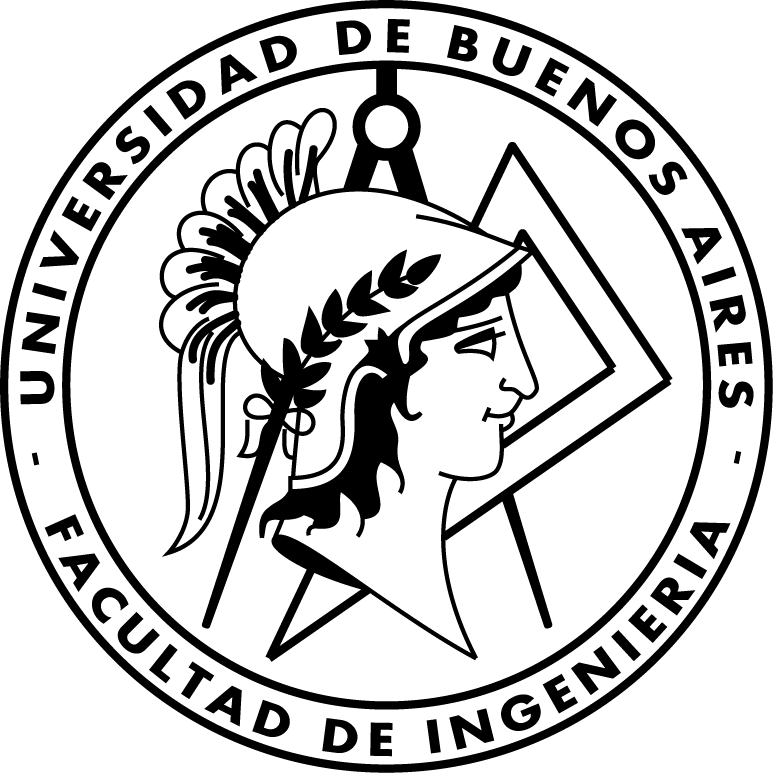
\includegraphics[scale=0.8]{images/logo-fiuba.png} \\
	\begin{center}	
		\textbf{Trabajo Práctico N$^{\circ}$1} \linebreak
 	\end{center}
	\begin{center}
		\begin{large}
			75.29 - Teoría de Algoritmos I \linebreak
			Facultad de Ingeniería de la Universidad de Buenos Aires \linebreak
			1er. Cuatrimestre 2017 \linebreak
		\end{large}
	\end{center} 
}
\author{	Federico Brasburg, \textit{Padrón Nro. 96.653}                     \\
            \texttt{ federico.brasburg.@gmail.com }                                              \\[2.5ex]
            Pablo Rodrigo Ciruzzi, \textit{Padrón Nro. 95.748}                     \\
            \texttt{ p.ciruzzi@hotmail.com }                                              \\[2.5ex]
            Andrés Otero, \textit{Padrón Nro. 96.604 }                     \\
            \texttt{ oteroandres95@gmail.com }                                              \\[2.5ex] \\
            \\
       }
\date{24 de abril de 2017}

\maketitle
\thispagestyle{empty}

\pagebreak 

\tableofcontents
\pagebreak

\clearpage
\section{Asignación de residencias}

\subsection{Reducción}
	Para reducir el problema de asignación de residencias al de matrimonios estables decidimos tomar algunas hipótesis para simplificar el problema y hacer más fácil la reducción. Las hipótesis son que el número de hospitales debe ser menor o igual al de residentes, así todos los hospitales tienen una vacante. El problema es que distintos hospitales tienen diferente cantidad de vacantes entonces para reducirlo hicimos que se modele cada vacante como un hospital diferente que tiene el mismo “ranking” que el hospital de la vacante de esa manera se vuelve un problema de n estudiantes contra $\sum_{i=0}^{|Q|-1} Q[i]$ hospitales (o vacantes).
    
\subsection{Resultados}
	\noindent El problema de asignación n = m = 100 tardó 0.00866603851318 segundos \\
	El problema de asignación n = m = 1000 tardó 0.756355047226 segundos \\
	El problema de asignación n = m = 10000 tardó 85.6384279728 segundos \\
	El problema de asignación n = m = 100000 no se corrió

\subsection{Conclusiones}
	El primer comentario a hacer es la no realización de n = m = 100000; se empezó corriendo pero se notaron problemas para hacerlo. Luego recurrimos a hacer las cuentas para dimensionar el problema y, al ser uno de 100000x100000, se necesitarían 10.000 millones de enteros para dimensionar una de las matrices de rankings. Es por ello que se decidió no realizar esta iteración del problema.
	\par En cuanto al rendimiento respecto al crecimiento del problema, vale la pena observar que el orden del problema \emph{O(n\textsuperscript{2})} coincide con el crecimiento de los tiempos respecto del orden de n, es decir, subiendo un orden el n se puede apreciar que sube 2 ordenes el tiempo utilizado. Podemos arriesgar que el problema más grande que no pudimos realizar estaría en el orden de 2 horas y media, suponiendo que el rendimiento fuera igual al de los anteriores. 	

\subsection{Conclusiones}
	Para crear y resolver un problema, se puede simplemente usando el script \texttt{correr\_asignacion.py} en la carpeta src. Para saber como usarlo correr \texttt{python correr\_asignacion.py $-$h}.

\section{Puntos de falla}
\subsection{Resultados}
	%\noindent Con 7 vértices y 16 aristas, tardó: 0.000223875045776 segundos \\
	\noindent Con 10 vértices y 20 aristas, tardó: 0.000194072723389 segundos \\
	Con 100 vértices y 200 aristas, tardó: 0.00134420394897 segundos \\
	Con 1000 vértices y 2000 aristas, tardó: 0.015242099762 segundos \\
	Con 10000 vértices y 20000 aristas, tardó: 0.146757125854 segundos \\
	Con 100000 vértices y 200000 aristas, tardó: 2.14698195457 segundos \\
	Con 1000000 vértices y 2000000 aristas, tardó: 25.5380079746 segundos \\
	\par Cabe aclarar que la cantidad de aristas está multiplicada por 2 ya que en nuestro modelo una arista no dirigida se corresponde a 2 aristas dirigidas.
	\par Aquí no aparece como resultado, pero se agregó un grafo de 7 vértices analizado en el curso, dando dos numeraciones distintas a los vértices para comprobar el buen funcionamiento del algoritmo ante el caso de una raíz con más de un hijo. Estos se encuentra en los archivos \texttt{g0.txt} y \texttt{g7.txt}.
\subsection{Funcionamiento}
	Cabe mencionar que en un primer momento el algoritmo se hizo de forma recursiva. El problema surgió cuando de esta manera, para los problemas más grandes, se excedía la cantidad de llamadas recursivas posibles dentro de Python. Por ello se tuvo que pasar a una forma iterativa del mismo.
	\par El funcionamiento en sí del algoritmo es bastante simple y se basa en recorridos DFS de un grafo. Lo que se hace es hacer un primer DFS para asignar el orden de visita de los nodos. Luego, utilizando este recorrido (modelado en una pila en nuestro caso), se asignan los valores de bajo para cada nodo. En este segundo recorrido, haciendo algunas comparaciones con este valor, se obtienen los vértices que son puntos de articulación.
	\par Por último, al terminar de recorrer un árbol DFS, se contempla el caso especial de la raíz, el cual se debe ver si tiene 2 o más hijos dentro del árbol para ver si es realmente punto de articulación o no.
\subsection{Conclusiones}
	Lo más importante a destacar es que se puede notar el orden lineal del algoritmo (\emph{O(|V|+|E|)}) mirando los tiempos de ejecución. Es simple ver cómo, cuando se aumenta en 1 el orden de magnitud de la entrada, lo mismo sucede con el tiempo de ejecución.
\subsection{Cómo correrlo}
	Para resolver los problemas brindados por el curso, basta con correr \texttt{python puntos\_articulacion.py}.

\section{Comunidades en redes}
\subsection{Algoritmo}
	Para está parte del práctico, se implementó el algoritmo de Kosaraju, que dado un grafo G dirigido, las componentes fuertemente conexas de G de la siguiente manera:
	\begin{itemize}
		\item Realiza un DFS a G y almacena el tiempo de finalizado de los vértices.
		\item Traspone G
		\item Realiza un DFS a G traspuesta respetando el orden de forma descendiente del tiempo de finalizado almacenado cuando se requiera decidir por cual vértice seguir.
	\end{itemize}
\subsection{Resultados}
	\noindent Con 10 vertices y 20 aristas, tardo: 0.000113964080811 segundos \\
	Con 100 vértices y 250 aristas, tardó: 0.00108599662781 segundos \\
	Con 1000 vértices y 2500 aristas, tardó: 0.0141451358795 segundos \\
	Con 10000 vértices y 25000 aristas, tardó: 0.148002147675 segundos \\
	Con 100000 vértices y 250000 aristas, tardó: 2.38693785667 segundos \\
	Con 1000000 vértices y 2500000 aristas, tardó: 31.3342020512 segundos
\subsection{Conclusiones}
    Se puede ver en los resultados que el orden del algoritmo de Kosaraju, que es \emph{O(|V|+|E|)} al estar implementado con un diccionario, es lineal y el orden crecimiento en tiempo del algoritmo implementado también es lineal. Finalmente, se comprobó que el orden lineal del algoritmo es correcto.
\subsection{Cómo correrlo}
	Correr la resolución de los problemas de componentes fuertemente conexas es tan simple como correr \texttt{python CFC.py}.

\pagebreak

\newpage
\section{Código}
\lstset{
	language=Python, columns=flexible, breaklines=true, frame=single, title=asignacion\_de\_residencias.py
}
\lstinputlisting{../src/asignacion_de_residencias.py}

\lstset{ title=CFC.py }
\lstinputlisting{../src/CFC.py}

\lstset{ title=correr\_asignacion.py }
\lstinputlisting{../src/correr_asignacion.py}

\lstset{ title=dfs.py }
\lstinputlisting{../src/dfs.py}

\lstset{ title=dfs\_iterativo.py }
\lstinputlisting{../src/dfs_iterativo.py}

\lstset{ title=grafo.py }
\lstinputlisting{../src/grafo.py}

\lstset{ title=parser.py }
\lstinputlisting{../src/parser.py}

\lstset{ title=puntos\_articulacion.py }
\lstinputlisting{../src/puntos_articulacion.py}

\lstset{ title=resultado\_DFS.py }
\lstinputlisting{../src/resultado_DFS.py}

\lstset{ title=tiempo.py }
\lstinputlisting{../src/tiempo.py}

\end{document}